\chapter {Análisis del sistema}

\section{Casuísticas que se dan y como se resuelve cada una}
		\begin{itemize}
			\item \textbf{Problema 1}: \textit{Recreación ante fallo total o réplica de infraestructura}. Ante un fallo total de la infraestructura o replicación para propósitos de testing, con los sistemas actuales sería imposible, ya que dada la configuración manual de cada uno de los servidores, sería imposible replicar al 100\% el estado de los servidores. 
			
			\item \textbf {Solución 1}: Al adoptar IaaC, la infraestructura estará codificada en ficheros de configuración bajo control de versiones. Pudiendo recrear la infraestructura bajo demanda en cualquier momento y asegurándonos de que sea la misma al 100%.
			
			\item \textbf{Problema 2}: \textit{Diferencias entre servidor de desarrollo y producción}. Al desarrollar en local, los desarrolladores no tienen una réplica de los servidores de producción para poder probar sus cambios. Esto hace que haya discrepancias entre Sistemas y desarrolladores puesto que puede funcionar en local con una configuración dada pero no en producción. 
			
			\item \textbf {Solución 2}: Al estar la infraestructura de cada aplicación codificada y bajo control de versiones, será sencillo replicar el entorno de producción en un entorno test para el desarrollo de aplicaciones.
			
			\item \textbf{Problema 3}: \textit{Petición de subidas a producción}. Al no existir cauces de integración o despliegue, no se tiene un conocimiento exacto de qué comportamiento va a tener la aplicación en producción. Esto y la necesidad de hacer peticiones al equipo de sistemas para subir nuevas versiones a producción ralentizan el desarrollo del software.
			
			\item \textbf{Solución 3:} Al tener el desarrollador un servidor réplica de producción para desplegar las aplicaciones, sabe perfectamente el comportamiento que va a tener en producción, puesto que son entornos idénticos. Esto y los cauces CI-CD solucionan el problema.
			
			\item \textbf{Problema 4}: \textit{Desconocimiento estado infraestructura o servicios}. Al configurarse los servidores de forma manual, parche tras parche, es imposible conocer en qué estado se encuentra la infraestructura. También dificulta la replicación de esta para procesos de pruebas.
			
			\item \textbf{Solución 4:} Misma solución que Problema 1. Al adoptar IaaC, la infraestructura estará codificada en ficheros de configuración bajo control de versiones. Esto facilita saber qué paquetes hay instalados en el sistema y qué configuración se ha desplegado para cada servicio.	
		\end{itemize}

\section{Metodología de desarrollo}
\begin{text}
	Todo proyecto software debe tener una organización y unas etapas de desarrollo bien definidas. En esta sección se pretende explicar la metodología de desarrollo elegida para realizar este proyecto. \\
	Se ha tratado este proyecto como cualquier otro proyecto software. Para la organización y el control de versiones se ha elegido Github, un software basado en git originalmente creado para el control de versiones. Actualmente, GitHub ofrece múltiples servicios, como almacenamiento, gestión de paneles de trabajo, registry, integración con múltiples tecnologías... \\
	En cuanto a la metodología de desarrollo, se ha optado por un desarrollo basado en Milestones. Cada Milestone está compuesto por Issues y estos están etiquetados y asignados a personas. A continuación se explican con mayor detalle estos conceptos.
\end{text}

\subsection{Milestones}
\label{milestones}
\begin{text}
	Los Milestones o Hitos en castellano, corresponden con estados finales deseados de la aplicación. Sabiendo esto, podríamos crear un Milestone por ejemplo: "Servidores configurados a través de ficheros de configuración Ansible". Esto será un estado final deseado para nuestra aplicación o proyecto. Para que un hito quede totalmente realizado, deben estar completos todos los issues marcados como esenciales para el hito. Un hito está compuesto por issues. A continuación se muestran algunos milestones creados en este proyecto, en el panel de administración GitHub.
	
	\begin{figure}[!hbt]
		\centering
		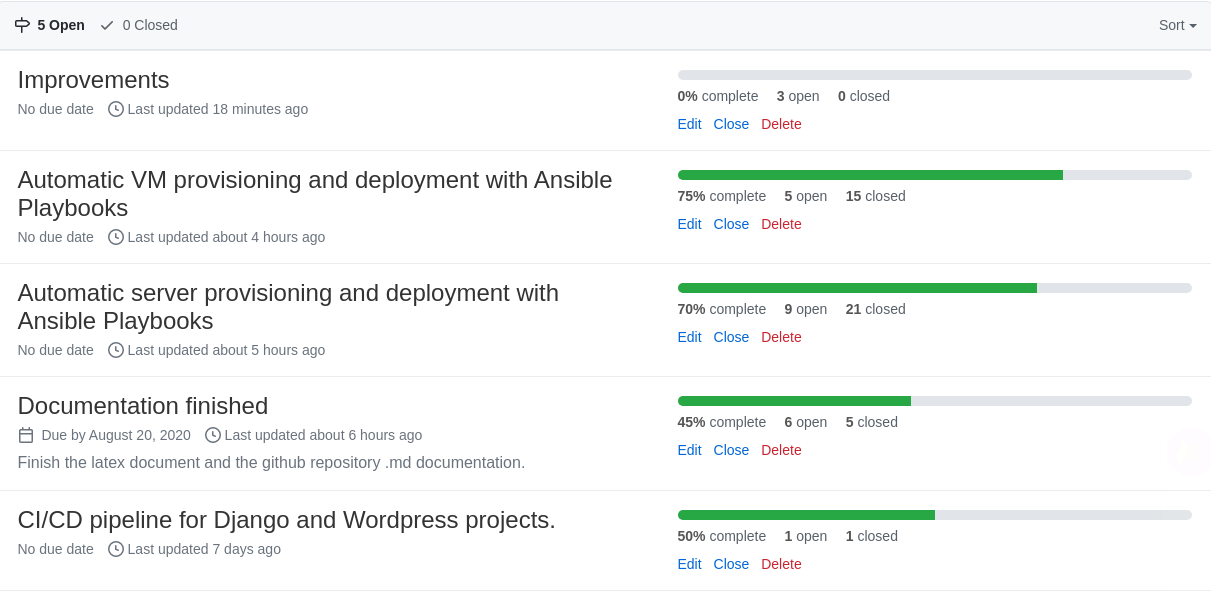
\includegraphics[scale=0.37]{imagenes/Analisis/milestones.png}
		\caption[GitHub milestones]{GitHub milestones}
		\label{github_milestones}
	\end{figure}
\end{text}
\subsection{Issues}
\begin{text}
	Como ya hemos visto, los issues forman parte de los hitos. Es una forma de desgranar el problema. Siguiendo el ejemplo anterior, si tenemos un hito: "Servidores configurados a través de ficheros de configuración Ansible", podemos desgranar el siguiente en distintos issues, que serían tareas más sencillas que hay que realizar para completar el hito. Por ejemplo, algunos issues serían: 
	\begin{itemize}
		\item Crear estructura directorios Ansible.
		\item Instalar paquetes en servidor a través de ficheros de configuración Ansible. \textbf{Core}
		\item Configurar interfaces de red a través de ficheros de configuración Ansible. \textbf{Core}
		\item Instalar ISO en servidor a través de ficheros de configuración Ansible. \textbf{Core}
		\item Instalar certificados SSL a través de ficheros de configuración Ansible. \textbf{Mejora}
	\end{itemize}
	
	Y así seguiríamos creando issues según creamos que van a ser necesarios para completar el hito en cuestión. \\
	En la sección  \nameref{milestones} hemos hablado que los issues tienen etiquetas. En la lista anterior por ejemplo, únicamente tenemos dos etiquetas que nos indican en este caso si son issues imprescindibles para el hito o simplemente mejoras. Gracias a estas etiquetas, podemos distinguir entre distintos tipos de issues y asignar mayor o menos prioridad por etiqueta. También gracias a Github, cada issue puede ser asignado a un desarrollador del proyecto. A continuación se muestra un ejemplo del panel de Github para mostrar los issues, etiquetas y hitos. \\
	Como se puede comprobar, el sistema de etiquetas y asignación de issues a desarrolladores, es más que suficiente para manejar proyectos. Permite asignar prioridades, agrupar issues en hitos y escribir comentarios en cada issue / Milestone. 
	
	\begin{figure}[!hbt]
		\centering
		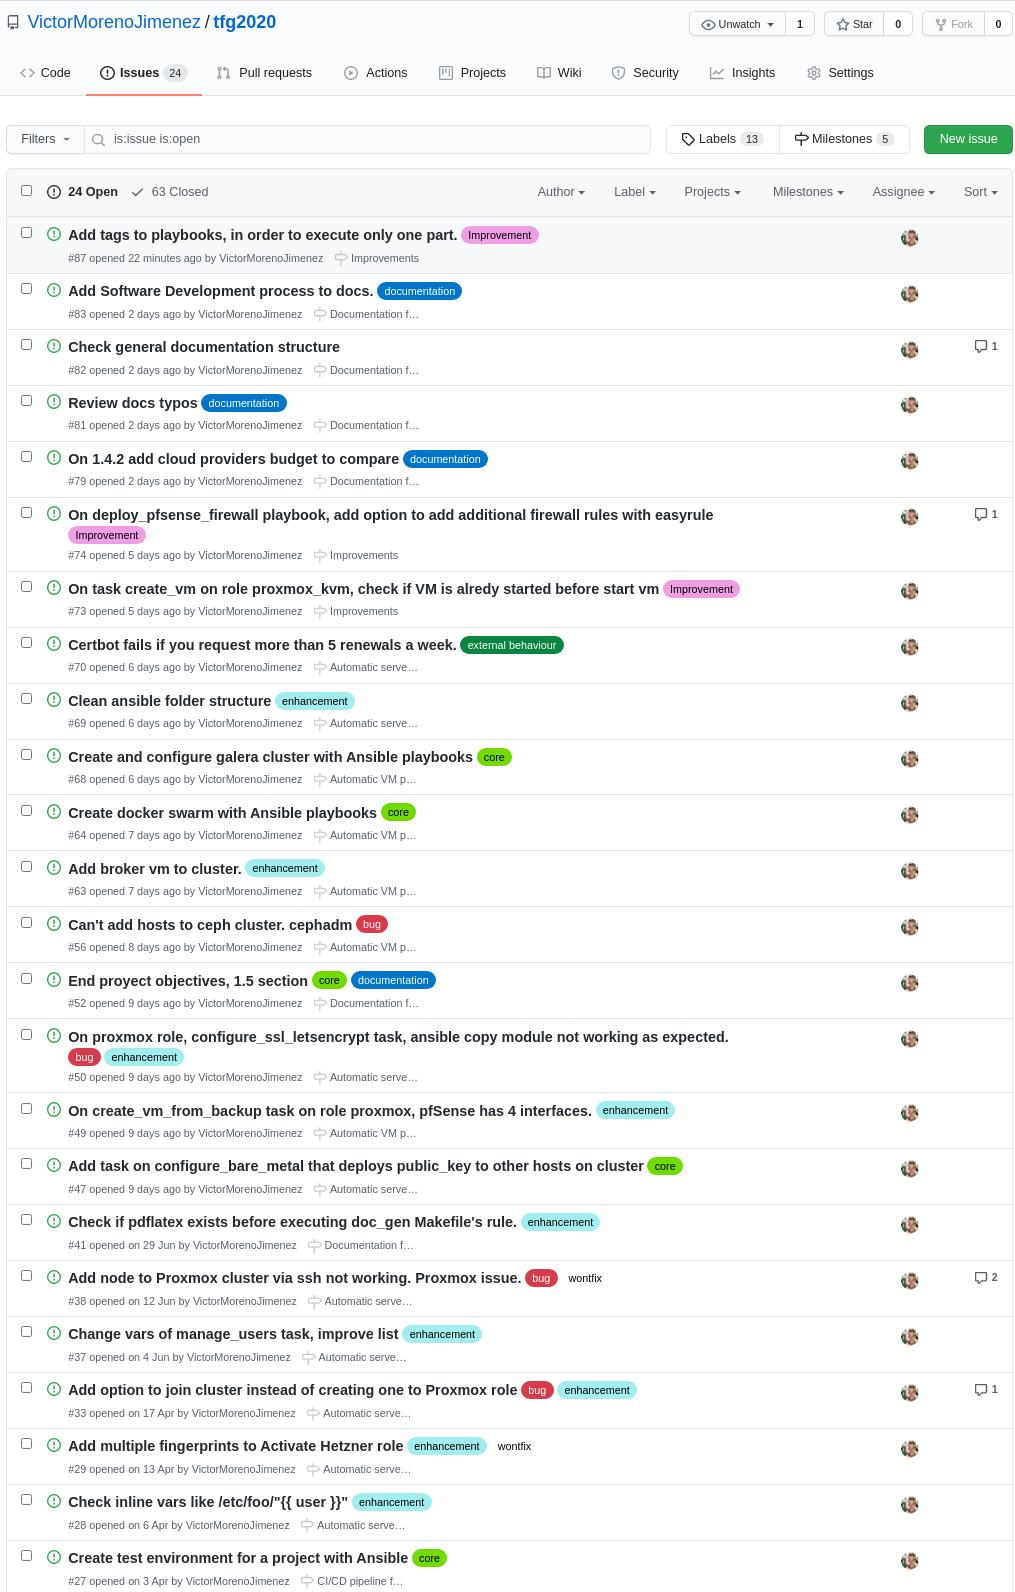
\includegraphics[scale=0.5]{imagenes/Analisis/githubissues.jpg}
		\caption[GitHub panel]{GitHub panel}
		\label{github_issues}
	\end{figure}
\end{text}
\clearpage

\section{Milestones, subjetivos, requisitos funcionales, restricciones e issues}
	\begin{text}
		En el capítulo 1, introducción se definen y detallan los objetivos que este proyecto pretende alcanzar. Sin embargo, estos objetivos presentan un alto grado de abstracción y es difícil trasladarlos a tareas concretas que se traducirán en issues del proyecto. En esta sección vamos a traducir los objetivos principales del proyecto en Milestones, desgranar los objetivos en subobjetivos y traducir cada subobjetivo a un requisito funcional que se convertirá en un issue en el proyecto.
	\end{text}

	\subsection{Milestones}
		\begin{text}
			Los Milestones son estados deseados del proyecto que queremos avanzar para completarlo. Cada Milestone termina un MVP (Minimum Viable Product) y cubre las necesidades de algún objetivo. A continuación se definen los Milestones y se agrupan por objetivos.
			
			\begin{itemize}
				\item \textbf{Milestone 0: Preparar entorno de desarrollo}. Antes de comenzar el proyecto, se debe configurar el equipo que se va a utilizar para trabajar, instalando y configurando el software necesario. 
				\item \textbf{Milestone 1:} Servicio de virtualización desplegado. 
				\item \textbf{Milestone 2:} Cluster seguro.
				\item \textbf{Milestone 3:} Control de versiones en cluster.
				\item \textbf{Milestone 4:} Cluster monitorizado.
				\item \textbf{Milestone 5:} Cluster preparado para desplegar aplicaciones.
				\item \textbf{Milestone 6:} Despliegue automático de aplicaciones.
			\end{itemize}
			A continuación se relaciona cada objetivo definido en la sección \nameref{objetivos_primarios} con su Milestone.
			
		
		\begin{table}[!hbt]
			\begin{tabular}{llllll}
				& Objetivo1         & Objetivo2         & Objetivo3         & Objetivo4         & Objetivo5         \\
				Milestone1 & \textbf{X} & \textbf{X} & \textbf{}  &            &            \\
				Mliestone2 & \textbf{X} & \textbf{X} &            &            &            \\
				Milestone3 &            &            & \textbf{X} & \textbf{X} &            \\
				Milestone4 &            &            & \textbf{X} & \textbf{X} &            \\
				Milestone5 &            &            & X          & \textbf{X} &            \\
				Milestone6 &            &            &            &            & \textbf{X}
			\end{tabular}
		\end{table}
	
		Los Milestones 1,2 están relacionados con la creación y replicación de la infraestructura base, mientras que los Milestones 3,4 y 5 con los servicios desplegados en la infraestructura. Milestone 6 asegura que existen cauces de integración continua y despliegue automático de aplicaciones.
			
		\end{text}

	\subsection{Subobjetivos}
		\begin{text}
			Vamos a analizar cada uno de los objetivos principales con el fin de desgranarlos en subobjetivos que se traduzcan en tareas realizables. 
			\begin{itemize}
				\item \textbf{Objetivo 1}. Asegurar unos tiempos bajos en la creación de infraestructura para proveer servicios.
				\begin{itemize}
					\item \textbf{Subobjetivo 1.1}. Automatización despliegue infraestructura sobre bare metal (tanto este subobjetivo como sus tareas se deben realizar de forma automática con alguna herramienta de automatización).
					\begin{itemize}
						\item Instalar ISO sobre bare metal.
						\item Configuración sistema.
						\item Instalar servicio de virtualización.
						\item Configurar servicio virtualización.
						\item Crear cluster usando el servicio de virtualización.
						\item Agregar los nodos al cluster.
						\item Configurar sistemas de almacenamiento en cluster.
					\end{itemize}
				\end{itemize}
				\item \textbf{Objetivo 2}. Replicar la infraestructura asegurando bajos tiempos de creación. El objetivo 1 cubre las necesidades del objetivo 2. Al crear la infraestructura con herramientas de automatización y estando la infraestructura codificada en ficheros de configuración bajo control de versiones, aseguramos poder replicar la infraestructura en cualquier momento. Al automatizarlo aseguramos mejores tiempos que de forma manual.
				
				\item \textbf{Objetivo 3}. Crear servicios necesarios para una empresa de aplicaciones web asegurando bajos tiempos de creación.
				\begin{itemize}
					\item \textbf{Subobjetivo 3.1}. Automatización despliegue servicios en infraestructura (tanto este subobjetivo como sus tareas se deben realizar de forma automática con alguna herramienta de automatización).
					\begin{itemize}
						\item Desplegar firewall redundante.
						\item Desplegar servicio de control de versiones.
						\item Desplegar servicio de almacenamiento estático.
						\item Desplegar servicio gestión aplicaciones.
						\item Desplegar servicio orquestación contenedores.
						\item Desplegar servicio de servidor web.
						\item Desplegar servicio de base de datos.
						\item Desplegar servicio de monitorización.
						\item Desplegar servicio gestor de colas.
					\end{itemize}
				\end{itemize}
				\item \textbf{Objetivo 4}. Replicar cualquier servicio alojado en la infraestructura de una empresa en la infraestructura de forma rápida. Al igual que pasa con los objetivos 1 y 2, los objetivos 3 y 4 están relacionados y si se cumple 3 se cumple 4. Si conseguimos automatizar la creación de los servicios con ficheros de configuración bajo control de versiones, aseguramos el poder replicarlos en cualquier momento.
				\item \textbf{Objetivo 5}. Crear cauces rápidos y seguros para la creación de nuevo software.
				\begin{itemize}
					\item \textbf{Subobjetivo 5.1}. Automatización despliegue aplicaciones con integración continua.
					\begin{itemize}
						\item Instalación y configuración servicio CI + CD.
						\item Adaptación proyecto a CI/CD (tests).
						\item Creación de los cauces en servicio elegido.
					\end{itemize}
				\end{itemize}
			\end{itemize}
		\end{text}
	
	\subsection{Requisitos funcionales}
	\begin{itemize}
		\item \textbf{RF 0.} El sistema permitirá la automatizar la configuración del equipo del sistema que va a utilizar el proyecto para la configuración de sistemas remotos.
		\item \textbf{RF 1.} El sistema permitirá la automatizar la creación de la infraestructura.
		\begin{itemize}
			\item \textbf{RF 1.1}. El sistema permitirá automatizar ĺa instalación de una ISO elegida sobre el servidor.
			\item \textbf{RF 1.2}. El sistema permitirá automatizar ĺa instalación de una ISO elegida sobre el servidor.
			\item \textbf{RF 1.3}. El sistema permitirá la instalación de un servicio de virtualización. 
			\item \textbf{RF 1.4}. El sistema permitirá la configuración de un servicio de virtualización.
			\item \textbf{RF 1.5}. El sistema permitirá la creación de un cluster sobre el servicio de virtualización.
			\item \textbf{RF 1.6}. El sistema permitirá añadir nuevos nodos al cluster.
			\item \textbf{RF 1.7}. El sistema permitirá configurar los sistemas de almacenamiento utilizados por el cluster.
		\end{itemize}
		\item \textbf{RF 2.} El sistema permitirá la replicación de la infraestructura.
		\item \textbf{RF 3.} El sistema permitirá la creación de los servicios necesarios para una empresa de desarrollo web.
		\begin{itemize}
			\item \textbf{RF 3.1}. El sistema permitirá la creación de un servicio de firewall en el cluster. (RNF 4)
			\item \textbf{RF 3.2}. El sistema permitirá la creación de un servicio de control de versiones en el cluster.
			\item \textbf{RF 3.3}. El sistema permitirá la creación de un servicio de almacenamiento estático en el cluster.
			\item \textbf{RF 3.4}. El sistema permitirá la creación de un servicio de gestión de aplicaciones Wordpress en el cluster.
			\item \textbf{RF 3.5}. El sistema permitirá la creación de un servicio de orquestación de contenedores en el cluster. (RNF 4)
			\item \textbf{RF 3.6}. El sistema permitirá la creación de un servicio de servidor web en el cluster.
			\item \textbf{RF 3.7}. El sistema permitirá la creación de un servicio de monitorización en el cluster.
			\item \textbf{RF 3.8}. El sistema permitirá la creación de un servicio de base de datos en el cluster. (RNF 3)
			\item \textbf{RF 3.9}. El sistema permitirá la creación de un servicio de gestión de colas.
		\end{itemize}
	
	\item \textbf{RF 4}. El sistema permitirá la recreación de infraestructura en un tiempo bajo.
	
	\item \textbf{RF 5}. El sistema permitirá el despliegue automatizados en un cluster seguro.
	\end{itemize}

	\subsection{Requisitos funcionales}
	\begin{itemize}
		\item \textbf{RNF 1}. El sistema debe garantizar la automatización de los procesos de creación de infraestructura.
		\item \textbf{RNF 2}. El sistema debe garantizar la automatización de los procesos de creación de servicios en la infraestructura.
		\item \textbf{RNF 3}. El sistema debe garantizar la alta disponibilidad de el servicio de base de datos.
		\item \textbf{RNF 4}. El sistema debe garantizar la alta disponibilidad de las aplicaciones.
	\end{itemize}

	\subsection{Restricciones}
	\begin{text}
		Este proyecto se ha desarrollado para una empresa en concreto y se realiza sobre una base. Esto conlleva restricciones a la hora de elegir las tecnologías a utilizar para satisfacer los objetivos. A continuación se listan las restricciones tecnológicas que presenta este proyecto.
		
		\begin{itemize}
			\item \textbf{Restricción 1.} El uso de las siguientes tecnologías será necesario para la correcta adaptación del proyecto a la empresa:
			\begin{itemize}
				\item Bases de datos: MySQL
				\item Almacenamiento estático: Ceph cluster
				\item Servicio virtualización: Proxmox
				\item Servido web: Nginx
				\item Contenedores: Docker
				\item Firewall: pfSense
				\item Control de versiones: GitLab
				\item Proyectos: Django + Angular \& Wordpress
			\end{itemize}
		\end{itemize}
	\end{text}

	\subsection{Tecnologías elegidas}
	\begin{text}
		Las tecnologías que se van a utilizar en la infraestructura y los servicios de el proyecto están bien definidas y son una restricción impuesta por la empresa, sin embargo para lograr el objetivo de este proyecto, hace falta elegir la herramienta de automatización que se va a elegir. A continuación se va a hacer un análisis de las principales herramientas disponibles, pros y contras de cada una y el por qué se ha elegido la tecnología utilizada.
	\end{text}
	\subsubsection{Puppet}
	\begin{text}
		Puppet es una herramienta de software libre de gestión de configuración de software. Es comúnmente utilizado por los administradores de sistemas para configurar múltiples servidores y para automatizar las tareas de mantenimiento. Puppet se adapta perfectamente a las necesidades de este proyecto. Sin embargo, la complejidad del lenguaje ruby junto con la necesidad de crear una infraestructura maestro - esclavo con los distintos nodos hace que se haya desechado esta opción.
	\end{text}
\clearpage
	\subsubsection{Chef}
	\begin{text}
		Chef es una herramienta open source con objetivos similares a Puppet. Basado en ruby y orientado a desarrolladores con experienca en ruby. La curva de aprendizaje es menor que la de Puppet. Sin embargo, también hay que crear una infraestructura específica para usar Chef con un nodo que actuaria de servidor y los nodos esclavos que serían los servidores a configurar.
	\end{text}
	\subsubsection{Ansible}
	\begin{text}
		Por último la elegida, Ansible. Ansible está basado en python y también es software libre. La gran ventaja de Ansible frente a Chef o Puppet es que no necesitamos generar ninguna estructura específica dentro del sistema para ejecutar tareas de Ansible. Simplemente instalar Ansible y los módulos necesarios según nuestras necesidades. También aprender Ansible es bastante asequible ya que los playbooks o ficheros de configuración Ansible son ficheros .yml. Los playbooks se ejecutan en orden secuencial lo que facilita mucho su comprensión. Es por todo esto que hemos elegido Ansible como herramienta de automatización para cumplir con los objetivos de este proyecto.
	\end{text}
	
	\subsection{Issues}
	\begin{text}
		A continuación se van a redactar los issues necesarios para cumplir con los requisitos funcionales. Se van a agrupar estos issues en Milestones.
		
		\begin{itemize}
			\item \textbf{Milestone 0:} Entorno de desarrollo. 
				\begin{itemize}
					\item \textbf{Issue 0.1}. Crear playbooks de Ansible para configurar el equipo de desarrollo.
					\item \textbf{Issue 0.2} Crear playbooks de Ansible para crear la estructura de carpetas necesaria para el proyecto.
				\end{itemize}
			\item \textbf{Milestone 1:} Servicio de virtualización desplegado. 
				\begin{itemize}
					\item \textbf{Issue 1.1}. Automatizar instalación ISO en servidores Hetzner con rescue mode activado.
					\item \textbf{Issue 1.2}. Automatizar configuración LVM sobre ISO instalada.
					\item \textbf{Issue 1.3}. Automatizar instalación paquetes en los nodos.
					\item \textbf{Issue 1.4}. Automatizar gestión de usuarios/grupos del sistema en los nodos.
					\item \textbf{Issue 1.5}. Automatizar la instalación de servicio de virtualización Proxmox en los nodos.
					\item \textbf{Issue 1.6}. Automatizar gestión de usuarios/grupos Proxmox en los nodos.
					\item \textbf{Issue 1.7}. Automatizar gestión de almacenamiento Proxmox en los nodos.
					\item \textbf{Issue 1.8}. Automatizar creación e instalación certificado SSL en los nodos.
					\item \textbf{Issue 1.9}. Automatizar la creación del cluster Proxmox.
					\item \textbf{Issue 1.10}. Automatizar la adición de nuevos nodos al cluster.
				\end{itemize}
			\item \textbf{Milestone 2:} Cluster seguro.
				\begin{itemize}
					\item \textbf{Issue 2.1}. Automatizar creación de máquina virtual pfSense en servicio de virtualización Proxmox.
					\item \textbf{Issue 2.2}. Modificar puerto SSH para poder ejecutar playbook sobre pfSense.
					\item \textbf{Issue 2.3}. Automatizar la configuración del firewall pfSense.
					\item \textbf{Issue 2.4}. Permitir la modificación de la configuración pfSense a través de un playbook de Ansible.
				\end{itemize}
			\item \textbf{Milestone 3:} Control de versiones en cluster.
				\begin{itemize}
					\item \textbf{Issue 3.1}. Automatizar la creación de máquina virtual en cluster donde instalar GitLab.
					\item \textbf{Issue 3.2}. Automatizar instalación GitLab en máquina virtual Proxmox.
					\item \textbf{Issue 3.3}. Automatizar configuración pfSense DHCP, añadir nueva IP.
					\item \textbf{Issue 3.4}. Automatizar configuración GitLab mediante ficheros de configuración.
				\end{itemize}
			\item \textbf{Milestone 4:} Cluster monitorizado.
				\begin{itemize}
					\item \textbf{Issue 4.1}. Automatizar la creación de máquina virtual en cluster donde instalar Icinga2.
					\item \textbf{Issue 4.2}. Automatizar instalación Icinga2 en máquina virtual Proxmox.
					\item \textbf{Issue 4.3}. Automatizar configuración pfSense DHCP, añadir nueva IP.
					\item \textbf{Issue 4.4}. Automatizar instalación Icinga2 Director sobre Icinga 2.
				\end{itemize}
			\item \textbf{Milestone 5:} Cluster preparado para desplegar aplicaciones.
				\begin{itemize}
					\item \textbf{Issue 5.1}. Automatizar instalación y configuración de Ceph cluster.
					\item \textbf{Issue 5.2}. Automatizar instalación y configuración der Galera cluster.
					\item \textbf{Issue 5.3}. Automatizar instalación y configuración de Virtualmin.
					\item \textbf{Issue 5.4}. Automatizar instalación y configuración de Kubernetes cluster.
					\item \textbf{Issue 5.5}. Automatizar instalación y configuración de RabbitMQ.
					\item \textbf{Issue 5.6}. Automatizar instalación y configuración de Nginx.
				\end{itemize}
			\item \textbf{Milestone 6:} Despliegue automático de aplicaciones.
				\begin{itemize}
					\item \textbf{Issue 6.1}. Dockerizar proyecto Django + Angular.
					\item \textbf{Issue 6.2}. Instalación y configuración de GiLab CI+CD.
					\item \textbf{Issue 6.3}. Adaptar proyecto a CI/CD.
				\end{itemize}
		\end{itemize}
	\end{text}

\clearpage
\section{Casos de uso}
	\subsection{CU 0. Configurar entorno proyecto}
	\begin{usecase}{Configurar entorno proyecto << CU.0 >>}
		\addrow{Descripción}{Configura el equipo donde se van a lanzar las tareas del proyecto.}
		
		\addrow{Actores}{Administrador/Desarrollador}
		
		\addrow{Precondición}{El usuario dispone de un equipo con una ISO instalada de la familia Debian.}
		
		\addrow{Postcondición}{El equipo del usuario queda preparado para la ejecución de tareas del proyecto.}
		
		\addmulrow{Secuencia principal (P)}{
			\item El usuario clona el proyecto
			\item El usuario configura las va- \\
			riables necesarias para ejecutar el \\ 
			playbook
			\item El usuario ejecuta el playbook \\ \textbf{configure\_development\_\\environment} 
			\item El sistema ejecuta las tareas en el \\
			equipo local
			\item El sistema informa al usuario \\
			del resultado de la ejecución}
		\hline
	\end{usecase}
	\clearpage
	\subsection{CU 0.1. Crear infraestructura}
	\begin{usecase}{Crear infraestructura << CU.1 >>}
		\addrow{Descripción}{Permite crear la infraestructura sobre los nodos.}
		
		\addrow{Actores}{Administrador}
		
		\addrow{Precondición}{El usuario administrador ha clonado el proyecto y ha configurado correctamente los ficheros hosts.yml, asignado valor a las variables de los roles hetzner y proxmox\_nodes y ejecutado caso de uso 0}
		
		\addrow{Postcondición}{Los nodos están configurados con la ISO elegida instalada y el servicio de virtualización Proxmox desplegado. Creado y configurado cluster Proxmox.}
		
		\addmulrow{Secuencia principal (P)}{
			\item El administrador clona el proyecto
			\item El administrador configura las va- \\
				riables necesarias para ejecutar el \\ 
				playbook
			\item El administrador ejecuta el play- \\
			book \textbf{configure\_proxmox\_nodes} 
			\item El sistema ejecuta las tareas en los \\
				nodos 
			\item El sistema informa al administrador \\
				  del resultado de la ejecución}
			  \hline
	\end{usecase}
	\clearpage
	\subsection{CU.2. Replicar infraestructura}
	\begin{usecase}{Replicar infraestructura << CU.2 >>}
		\addrow{Descripción}{Permite replicar la infraestructura sobre los nodos.}
		
		\addrow{Actores}{Administrador}
		
		\addrow{Precondición}{El usuario administrador ha clonado el proyecto y ha configurado correctamente el fichero hosts.yml con los nuevos nodos donde replicar la infraestructura, asignado valor a las variables de los roles hetzner y proxmox\_nodes y ejecutado caso de uso 0}
		
		\addrow{Postcondición}{La infraestructura desplegada en << CU.1 >> queda replicada en los nodos elegidos.}
		
		\addmulrow{Secuencia principal (P)}{
			\item El administrador clona el proyecto
			\item El administrador configura las va- \\
			riables necesarias para ejecutar el \\ 
			playbook
			\item El administrador ejecuta el play- \\
			book \textbf{configure\_proxmox\_nodes} 
			\item El sistema ejecuta las tareas en los \\
			nodos 
			\item El sistema informa al administrador \\
			del resultado de la ejecución}
 
		\hline
	\end{usecase}
	\clearpage
	
	\subsection{CU.3. Crear servicio firewall}
	\begin{usecase}{Crear servicio firewall << CU.3 >>}
		\addrow{Descripción}{Permite crear un servicio de firewall en el cluster.}
		
		\addrow{Actores}{Administrador}
		
		\addrow{Precondición}{El usuario ha ejecutado correctamente << CU.0 >> y  << CU.1 >> o << CU.2 >>}
		
		\addrow{Postcondición}{Se ha creado el servicio de firewall pfSense en el cluster.}
		
		\addmulrow{Secuencia principal (P)}{
			\item El administrador ejecuta \\ correctamente << CU.0 >>
			\item El administrador ejecuta \\ correctamente  << CU.1 >> \\
			o << CU.2 >>.
			\item El administrador configura \\ variables 
			de role \textbf{pfsense} 
			\item El administrador ejecuta playbook \\  
				\textbf{deploy\_pfsense\_firewall}
			\item El sistema ejecuta las tareas en los \\
			nodos. 
			\item El sistema informa al administrador \\
			del resultado de la ejecución}
		\hline
	\end{usecase}
\clearpage
\subsection{CU.4. Crear servicio almacenamiento estático}
\begin{usecase}{Crear servicio almacenamiento estático << CU.4 >>}
	\addrow{Descripción}{Permite crear un servicio de almacenamiento estático en el cluster.}
	
	\addrow{Actores}{Administrador}
	
	\addrow{Precondición}{El usuario ha ejecutado correctamente << CU.0 >> y  << CU.1 >> o << CU.2 >> y << CU.3 >>}
	
	\addrow{Postcondición}{Se ha creado el servicio de almacenamiento estático \textbf{Ceph cluster} en el cluster.}
	
	\addmulrow{Secuencia principal (P)}{
		\item El administrador ejecuta \\ correctamente << CU.0 >>
		\item El administrador ejecuta \\ correctamente  << CU.1 >> \\
		o << CU.2 >> y << CU.3 >>.
		\item El administrador configura \\ variables 
		de role \textbf{pfsense} 
		\item El administrador ejecuta playbook \\  
		\textbf{deploy\_pfsense\_firewall}
		\item El sistema ejecuta las tareas en los \\
		nodos. 
		\item El sistema informa al administrador \\
		del resultado de la ejecución}
	\hline
\end{usecase}

\subsection{CU.5. Crear servicio de gestión de aplicaciones Wordpress}
\begin{usecase}{Crear servicio de gestión de aplicaciones Wordpress << CU.5 >>}
	\addrow{Descripción}{Permite crear un servicio de gestión de aplicaciones Wordpress en el cluster.}
	
	\addrow{Actores}{Administrador}
	
	\addrow{Precondición}{El usuario ha ejecutado correctamente << CU.0 >> y  << CU.1 >> o << CU.2 >> y << CU.3 >>}
	
	\addrow{Postcondición}{Se ha creado el servicio de gestión de aplicaciones Wordpress en el cluster.}
	
	\addmulrow{Secuencia principal (P)}{
		\item El administrador ejecuta \\ correctamente << CU.0 >>
		\item El administrador ejecuta \\ correctamente  << CU.1 >> \\
		o << CU.2 >> y << CU.3 >>.
		\item El administrador configura \\ variables 
		de role \textbf{virtualmin} 
		\item El administrador ejecuta playbook \\  
		\textbf{create\_virtualmin}
		\item El sistema ejecuta las tareas en los \\
		nodos. 
		\item El sistema informa al administrador \\
		del resultado de la ejecución}
	\hline
\end{usecase}

\clearpage 
\subsection{CU.6. Crear servicio de orquestación de contenedores en el cluster}
\begin{usecase}{Crear servicio de orquestación de contenedores en el cluster << CU.6 >>}
	\addrow{Descripción}{Permite crear un servicio de orquestación de contenedores en el cluster en el cluster.}
	
	\addrow{Actores}{Administrador}
	
	\addrow{Precondición}{El usuario ha ejecutado correctamente << CU.0 >> y  << CU.1 >> o << CU.2 >> y << CU.3 >>}
	
	\addrow{Postcondición}{Se ha creado el servicio de orquestación de contenedores en el cluster.}
	
	\addmulrow{Secuencia principal (P)}{
		\item El administrador ejecuta \\ correctamente << CU.0 >>
		\item El administrador ejecuta \\ correctamente  << CU.1 >> \\
		o << CU.2 >> y << CU.3 >>.
		\item El administrador configura \\ variables 
		de role \textbf{kubernetes} 
		\item El administrador ejecuta playbook \\  
		\textbf{create\_kubernetes\_cluster}
		\item El sistema ejecuta las tareas en los \\
		nodos. 
		\item El sistema informa al administrador \\
		del resultado de la ejecución}
	\hline
\end{usecase}

\clearpage
\subsection{CU.7. Crear servicio de monitorización en el cluster}
\begin{usecase}{Crear servicio de monitorización en el cluster << CU.7 >>}
	\addrow{Descripción}{Permite crear un servicio de monitorización en el cluster.}
	
	\addrow{Actores}{Administrador}
	
	\addrow{Precondición}{El usuario ha ejecutado correctamente << CU.0 >> y  << CU.1 >> o << CU.2 >> y << CU.3 >>}
	
	\addrow{Postcondición}{Se ha creado el servicio de monitorización en el cluster.}
	
	\addmulrow{Secuencia principal (P)}{
		\item El administrador ejecuta \\ correctamente << CU.0 >>
		\item El administrador ejecuta \\ correctamente  << CU.1 >> \\
		o << CU.2 >> y << CU.3 >>.
		\item El administrador configura \\ variables 
		de role \textbf{icinga2}.
		\item El administrador ejecuta playbook \\  
		\textbf{create\_icinga2}.
		\item El sistema ejecuta las tareas en los \\
		nodos. 
		\item El sistema informa al administrador \\
		del resultado de la ejecución}
	\hline
\end{usecase}

\clearpage
\subsection{CU.8. Crear servicio de bases de datos}
\begin{usecase}{Crear servicio de bases de datos << CU.8 >>}
	\addrow{Descripción}{Permite crear un servicio bases de datos en el cluster.}
	
	\addrow{Actores}{Administrador}
	
	\addrow{Precondición}{El usuario ha ejecutado correctamente << CU.0 >> y  << CU.1 >> o << CU.2 >> y << CU.3 >>}
	
	\addrow{Postcondición}{Se ha creado el servicio de bases de datos en el cluster.}
	
	\addmulrow{Secuencia principal (P)}{
		\item El administrador ejecuta \\ correctamente << CU.0 >>
		\item El administrador ejecuta \\ correctamente  << CU.1 >> \\
		o << CU.2 >> y << CU.3 >>.
		\item El administrador configura \\ variables 
		de role \textbf{icinga2} 
		\item El administrador ejecuta playbook \\  
		\textbf{create\_galera\_cluster}
		\item El sistema ejecuta las tareas en los \\
		nodos. 
		\item El sistema informa al administrador \\
		del resultado de la ejecución}
	\hline
\end{usecase}

\clearpage 
\subsection{CU.10. Crear servicio de gestión de colas}
\begin{usecase}{Crear servicio de gestión de colas << CU.10 >>}
	\addrow{Descripción}{Permite crear un servicio gestión de colas en el cluster.}
	
	\addrow{Actores}{Administrador}
	
	\addrow{Precondición}{El usuario ha ejecutado correctamente << CU.0 >> y  << CU.1 >> o << CU.2 >> y << CU.3 >>}
	
	\addrow{Postcondición}{Se ha creado el servicio de gestión de colas en el cluster.}
	
	\addmulrow{Secuencia principal (P)}{
		\item El administrador ejecuta \\ correctamente << CU.0 >>
		\item El administrador ejecuta \\ correctamente  << CU.1 >> \\
		o << CU.2 >> y << CU.3 >>.
		\item El administrador configura \\ variables 
		de role \textbf{rabbitmq} 
		\item El administrador ejecuta playbook \\  
		\textbf{create\_rabbitmq}
		\item El sistema ejecuta las tareas en los \\
		nodos. 
		\item El sistema informa al administrador \\
		del resultado de la ejecución}
	\hline
\end{usecase}

\clearpage
\subsection{CU.11. Recrear infraestructura}
\begin{usecase}{Recrear infraestructura << CU.11 >>}
	\addrow{Descripción}{Permite replicar infraestructura en nuevos nodos.}
	
	\addrow{Actores}{Administrador}
	
	\addrow{Precondición}{El usuario administrador ha ejecutado correctamente << CU.0 >>, los ficheros hosts.yml con los nodos objetivo y asignado las variables necesarias en os roles \textbf{hetzner}y \textbf{proxmox\_nodes}.}
	
	\addrow{Postcondición}{La infraestructura queda replicada en nuevos nodos.}
	
	\addmulrow{Secuencia principal (P)}{
	\item El administrador ejecuta \\ correctamente << CU.0 >>
	\item El administrador ejecuta \\ correctamente  << CU.1 >> \\
	o << CU.2 >> y << CU.3 >>.
	\item El administrador configura \\ variables 
	de role \textbf{proxmox\_kvm} 
	\item El administrador ejecuta playbook \\  
	\textbf{configure\_proxmox\_nodes}
	\item El sistema ejecuta las tareas en los \\
	nodos. 
	\item El sistema informa al administrador \\
	del resultado de la ejecución}
\hline
\end{usecase}
\clearpage 

\section{Arquitectura del Sistema}
	\subsection{Servidores Físicos}
		\begin{text}
			Al trabajar en una empresa de hosting, he tenido la suerte de contar con 3 servidores bare metal para el desarrollo de este proyecto. Las características técnicas de los servidores se pueden consultar en \nameref{servidores_bare_metal}.
		\end{text}
	\subsection{Infraestructura objetivo}
		\begin{text}
			Este proyecto pretende crear una infraestructura robusta para una pequeña empresa que se dedique al desarrollo del software. Ésta infraestructura debe ser robusta al igual que segura, con lo que ha de proporcionar firewalls redundantes y algún mecanismo para proporcional alta disponibilidad en las aplicaciones web.  A continuación se muestra la infraestructura objetivo.
		\end{text}
	
	\subsection{VSwitch}
	\begin{text}
		El cluster está bajo la red LAN 10.6.0.0/16, de forma que todas las máquinas virtuales están comunicadas. Sin embargo los nodos principales (tfg.intelligenia.com, tfg2.intelligenia.com y tfg3.intelligenia.com) tienen que estar comunicados a través de una red interna para el correcto funcionamiento de Proxmox y los pfSense.
		Es aquí donde entran en juego los switches virtuales de Hetzner. Un VSwitch simula el funcionamiento de un switch convencional, conectando los servidores que se conecten al switch entre sí. De este modo, conseguimos crear una red de conexión entre los nodos principales.
	\end{text}

	\begin{figure}[!hbt]
		\label{InfraestructuraObjetivo}
		\centering
		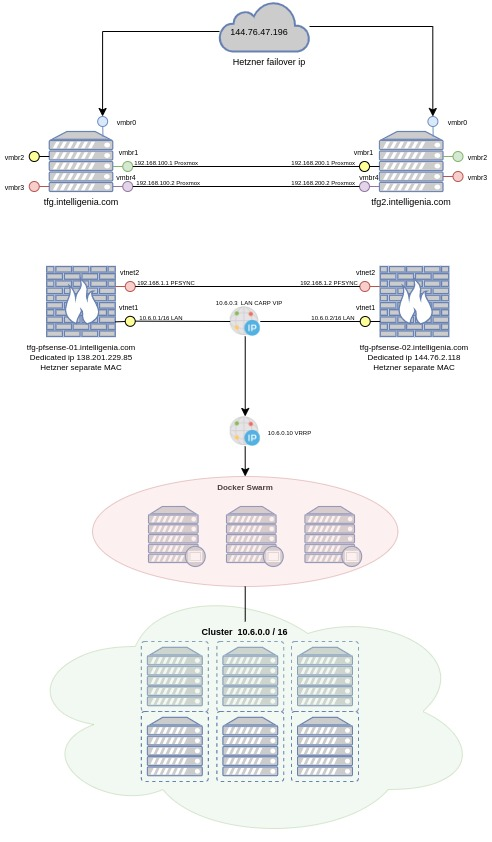
\includegraphics[scale=0.75]{imagenes/Analisis/diagrama.jpg}
		\caption[Infraestructura Objetivo]{Infraestructura Objetivo}
	\end{figure}

	\begin{figure}[!hbt]
		\centering
		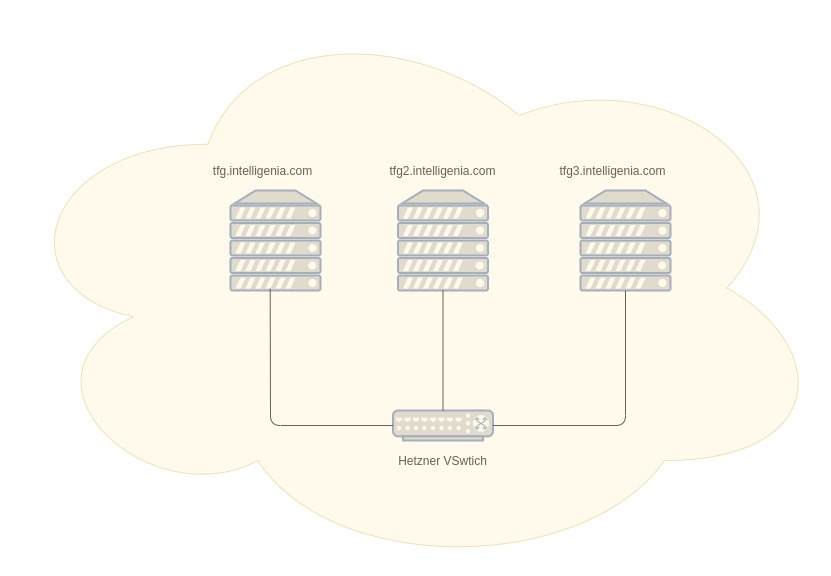
\includegraphics[scale=0.4]{imagenes/Analisis/vswitch.jpg}
		\caption[VSwitch]{VSwitch}
		\label{VSwitch}
	\end{figure}

	
	
	